\chapter{scanf()}
\index{\CStandardLibrary!scanf()}
\label{label_scanf}

\RU{Теперь попробуем использовать scanf().}\EN{Now let's use scanf().}

\lstinputlisting{patterns/04_scanf/ex1.c}

\RU{Да, согласен, использовать \scanf в наши времена для того, чтобы спросить у пользователя что-то, 
не самая хорошая идея.
Но я хотел проиллюстрировать передачу указателя на переменную типа \Tint.}
\EN{OK, I agree, it is not clever to use \scanf for user interactions today. 
But I wanted to illustrate passing pointer to \Tint type variable.}

\section{\RU{Об указателях}\EN{About pointers}}
\index{\CLanguageElements!\Pointers}

\RU{Это одна из фундаментальных вещей в компьютерных науках.}\EN{It is one of the most fundamental things in computer
science.}
\RU{Часто большой массив, структуру или объект передавать в другую функцию никак не выгодно, 
а передать её адрес куда проще.}
\EN{Often, large array, structure or object, it is too costly to pass to other function, 
while passing its address is much easier.}
\RU{К тому же, если вызываемая функция должна изменить что-то в этом большом массиве или структуре,
то возвращать её полностью ~--- это так же абсурдно.}
\EN{More than that: if calling function must modify something in the large array or structure,
to return it as a whole is absurd as well.}
\RU{Так что самое простое, что можно сделать, это передать в функцию адрес массива или структуры,
и пусть она что-то там изменит.}
\EN{So the simplest thing to do is to pass an address of array or structure to function,
and let it change what must be changed.}

\RU{Указатель в}\EN{In} \CCpp \RU{ ~--- это просто адрес какого-либо места в памяти.}
\EN{it is just an address of some point in memory.}

\index{x86-64}
\RU{В x86 адрес представляется в виде 32-битного числа (т.е., занимает 4 байта), а в x86--64 как 64-битное число 
(занимает 8 байт).}
\EN{In x86, address is represented as 32-bit number (i.e., occupying 4 bytes), while in x86--64 it is 64-bit number
(occupying 8 bytes).}
\RU{Кстати, отсюда негодование некоторых людей, связанное с переходом на x86-64 ~--- на этой архитектуре все указатели
будут занимать места в 2 раза больше.}
\EN{By the way, that is the reason of some people's indignation related to switching to x86-64~---all pointers
on x64-architecture will require twice as more space.}

\index{\CStandardLibrary!memcpy()}
\RU{При некотором упорстве можно работать только с бестиповыми указателями (\TT{void*})}\EN{With some effort,
it is possible to work only with untyped pointers}; \RU{например,}\EN{e.g.} 
\RU{стандартная функция Си}\EN{standard C function} \TT{memcpy()},
\RU{копирующая блок из одного места памяти в другое}\EN{copying a block from one place in memory to another}, 
\RU{принимает на вход 2 указателя типа}\EN{takes 2 pointers of} \TT{void*}\EN{ type on input}, 
\RU{потому что нельзя
заранее предугадать, какого типа блок вы собираетесь копировать. 
Да в общем это и не важно, важно только знать размер блока.}
\EN{since it is impossible to predict block data type you would like to copy. 
And it is not even important to know, only block size matters.}

\RU{Также указатели широко используются, когда функции нужно вернуть более одного значения}
\EN{Also pointers are widely used when function needs to return more than one value}
(\RU{мы еще вернемся к этому в будущем}\EN{we will back to this in future}~(\ref{label_pointers})).
\IT{scanf()} \RU{ ~--- это как раз такой случай}\EN{is just that case}. 
\RU{Помимо того, что этой функции нужно показать, сколько значений
было прочитано успешно, ей еще и нужно вернуть сами значения.}
\EN{In addition to the function's need to show how many values were read successfully, 
it also should return all these values.}

\RU{Тип указателя в}\EN{In} \CCpp \RU{нужен для проверки типов на стадии компиляции.}
\EN{pointer type is needed only for type checking on compiling stage.}
\RU{Внутри, в скомпилированном коде, никакой информации о типах указателей нет вообще.}
\EN{Internally, in compiled code, there is no information about pointer types at all.}

\section{x86}

\subsection{MSVC}

\RU{Что получаем на ассемблере компилируя MSVC 2010:}
\EN{What we got after compiling in MSVC 2010:}

\lstinputlisting{patterns/04_scanf/ex1_MSVC.asm}

\RU{Переменная \TT{x} является локальной.}\EN{Variable \TT{x} is local.} 

\RU{По стандарту \CCpp она доступна только из этой же функции и ниоткуда более. 
Так получилось, что локальные переменные располагаются в стеке. 
Может быть, можно было бы использовать и другие варианты, но в x86 это традиционно так.}
\EN{\CCpp standard tell us it must be visible only in this function and not from any other point. 
Traditionally, local variables are placed in the stack. 
Probably, there could be other ways, but in x86 it is so.}

\index{x86!\Instructions!PUSH}
\RU{Следующая после пролога инструкция \TT{PUSH ECX} не ставит своей целью сохранить 
значение регистра \ECX. 
(Заметьте отсутствие соответствующей инструкции \TT{POP ECX} в конце функции)}
\EN{Next instruction after function prologue, \TT{PUSH ECX}, has not a goal to save \ECX state 
(notice absence of corresponding \TT{POP ECX} at the function end).}

\RU{Она на самом деле выделяет в стеке 4 байта для хранения \TT{x} в будущем.} 
\EN{In fact, this instruction just allocates 4 bytes on the stack for \TT{x} variable storage.} 

\label{stack_frame}
\index{\Stack!\RU{Стековый фрейм}\EN{Stack frame}}
\index{x86!\Registers!EBP}
\RU{Доступ к \TT{x} будет осуществляться при помощи объявленного макроса \TT{\_x\$} 
(он равен -4) и регистра \EBP указывающего на текущий фрейм.}
\EN{\TT{x} will be accessed with the assistance of the \TT{\_x\$} macro 
(it equals to -4) and the \EBP register pointing to current frame.}

\RU{Вообще, во все время исполнения функции, \EBP указывает на текущий \glslink{stack frame}{фрейм} и через \TT{EBP+смещение}
можно иметь доступ как к локальным переменным функции, так и аргументам функции.} 
\EN{Over a span of function execution, \EBP is pointing to current \gls{stack frame} and it is possible 
to have an access to local variables and function arguments via \TT{EBP+offset}.}

\index{x86!\Registers!ESP}
\RU{Можно было бы использовать \ESP, но он во время исполнения функции постоянно меняется. 
Так что можно сказать, что \EBP это \IT{замороженное состояние} \ESP на момент начала исполнения функции.}
\EN{It is also possible to use \ESP, but it is often changing and not very convenient.
So it can be said, the value of the \EBP is \IT{frozen state} of the value of the \ESP at the moment of function execution start.}

\RU{Разметка типичного стекового \glslink{stack frame}{фрейма} в 32-битной среде}
\EN{A very typical \gls{stack frame} layout in 32-bit environment is}:

\begin{center}
\begin{tabular}{ | l | l | }
\hline
\dots & \dots \\
\hline
EBP-8 & \RU{локальная переменная}\EN{local variable} \#2, \MarkedInIDAAs{} \TT{var\_8} \\
\hline
EBP-4 & \RU{локальная переменная}\EN{local variable} \#1, \MarkedInIDAAs{} \TT{var\_4} \\
\hline
EBP & \RU{сохраненное значение}\EN{saved value of} \EBP \\
\hline
EBP+4 & \RU{адрес возврата}\EN{return address} \\
\hline
EBP+8 & \argument \#1, \MarkedInIDAAs{} \TT{arg\_0} \\
\hline
EBP+0xC & \argument \#2, \MarkedInIDAAs{} \TT{arg\_4} \\
\hline
EBP+0x10 & \argument \#3, \MarkedInIDAAs{} \TT{arg\_8} \\
\hline
\dots & \dots \\
\hline
\end{tabular}
\end{center}

\RU{У функции \scanf в нашем примере два аргумента.}\EN{Function \scanf in our example has two arguments.}

\RU{Первый ~--- указатель на строку содержащую \TT{``\%d''} и второй ~--- адрес переменной \TT{x}.} 
\EN{First is pointer to the string containing \TT{``\%d''} and second~---address of variable \TT{x}.} 

\index{x86!\Instructions!LEA}
\RU{Вначале адрес \TT{x} помещается в регистр \EAX при помощи инструкции \TT{lea eax, DWORD PTR \_x\$[ebp]}.}
\EN{First of all, address of the \TT{x} variable is placed into the \EAX register by \TT{lea eax, DWORD PTR \_x\$[ebp]} instruction}

\RU{Инструкция \LEA означает \IT{load effective address}, но со временем она изменила свою функцию}
\EN{\LEA meaning \IT{load effective address} but over a time it changed its primary application}
~(\ref{sec:LEA}).

\RU{Можно сказать, что в данном случае \LEA просто помещает в \EAX результат суммы значения в регистре 
\EBP и макроса \TT{\_x\$}.}
\EN{It can be said, \LEA here just stores sum of the value in the \EBP register and \TT{\_x\$} macro to the \EAX register.}

\RU{Это тоже что и}\EN{It is the same as} \TT{lea eax, [ebp-4]}.

\RU{Итак, от значения \EBP отнимается $4$ и помещается в \EAX.
Далее значение \EAX заталкивается в стек и вызывается \scanf.}
\EN{So, $4$ subtracting from value in the \EBP register and result is placed to the \EAX register.
And then value in the \EAX register is pushing into stack and \scanf is called.}

\RU{После этого вызывается \printf. Первый аргумент вызова которого, строка:} 
\EN{After that, \printf is called. First argument is pointer to string:} \TT{``You entered \%d...\textbackslash{}n''}.

\RU{Второй аргумент: \TT{mov ecx, [ebp-4]}, эта инструкция помещает в \ECX не адрес переменной \TT{x}, 
а его значение, что там сейчас находится.}
\EN{Second argument is prepared as: \TT{mov ecx, [ebp-4]},
this instruction places to the \ECX not address of the \TT{x} variable, but its contents.}

\RU{Далее значение \ECX заталкивается в стек и вызывается последний \printf.}
\EN{After, value in the \ECX is placed on the stack and the last \printf called.}

\subsection{MSVC + \olly}
\index{\olly}

\RU{Попробуем этот же пример в}\EN{Let's try this example in} \olly.
\RU{Загружаем, нажимаем F8 (\stepover) до тех пор, пока не окажемся в своем исполняемом файле,
а не в}\EN{Let's load, press F8 (\stepover) until we get into our executable file
instead of} \TT{ntdll.dll}.
\RU{Скроллим вверх, до тех пока не найдем \main}\EN{Scroll up until \main appears}.
\RU{Кликаем на первой инструкции}\EN{Let's click on the first instruction} (\TT{PUSH EBP}), 
\RU{нажимаем}\EN{press} F2, \RU{затем}\EN{then} F9 (Run) \RU{и брякпойнт срабатывает
на начале \main}\EN{and breakpoint triggers on the \main begin}.

\RU{Трассируем до того места, где готовится адрес переменной $x$}
\EN{Let's trace to the place where the address of $x$ variable is prepared}:
\figref{fig:scanf_ex1_olly_1}.

\RU{На \EAX в окне регистров можно нажать правой кнопкой и далее}
\EN{It is possible to right-click on \EAX in registers window and then} ``Follow in stack''.
\RU{Этот адрес покажется в окне стека}\EN{This address will appear in stack window}.
\RU{Смотрите, это переменная в локальном стеке}\EN{Look, this is a variable in the local stack}.
\RU{Я нарисовал там красную стрелку}\EN{I drawed a red arrow there}.
\RU{И там сейчас какой-то мусор}\EN{And there are some garbage} (\TT{0x77D478}).
\RU{Адрес этого элемента стека сейчас, при помощи \PUSH, запишется в этот же стек, рядом}
\EN{Now address of the stack element, with the help of \PUSH, will be written to the same stack, nearly}.
\RU{Трассируем при помощи F8 вплоть до конца исполнения \scanf}\EN{Let's trace by F8 until \scanf 
execution finished}.
\RU{А пока \scanf исполняется, в консольном окне, вводим, например, 123}
\EN{During the moment of \scanf execution, we enter, for example, 123, in the console window}:

\begin{figure}[H]
\centering
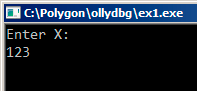
\includegraphics[scale=0.66]{patterns/04_scanf/ex1_olly_2.png}
\caption{\RU{Вывод в консоль}\EN{Console output}}
\label{fig:scanf_ex1_olly_2}
\end{figure}

\RU{Вот тут }\scanf \RU{отработал}\EN{executed here}: \figref{fig:scanf_ex1_olly_3}. 
\scanf \RU{вернул}\EN{returns} $1$ \InENRU \EAX, \RU{что означает, что он успешно прочитал одно 
значение}\EN{which means, it have read one value successfully}.
\RU{В наблюдаемом нами элементе стека теперь}\EN{The element of 
stack of our attention now contain} \TT{0x7B} (123).

\RU{Чуть позже, это значение копируется из стека в регистр \ECX и передается в \printf}
\EN{Further, this value is copied from the stack to the \ECX register and passed into \printf}:
\figref{fig:scanf_ex1_olly_4}.

\begin{figure}[H]
\centering
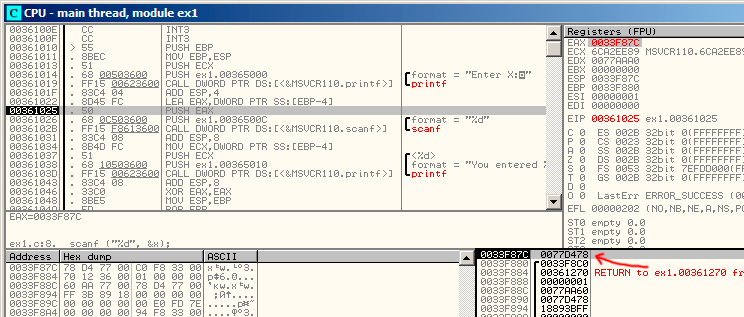
\includegraphics[scale=\FigScale]{patterns/04_scanf/ex1_olly_1.png}
\caption{\olly: \RU{вычисляется адрес локальной переменной}\EN{address of the local variable is computed}}
\label{fig:scanf_ex1_olly_1}
\end{figure}

\begin{figure}[H]
\centering
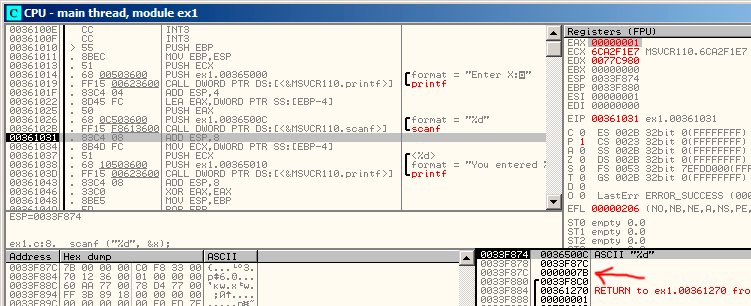
\includegraphics[scale=\FigScale]{patterns/04_scanf/ex1_olly_3.png}
\caption{\olly: \scanf \RU{исполнилась}\EN{executed}}
\label{fig:scanf_ex1_olly_3}
\end{figure}

\begin{figure}[H]
\centering
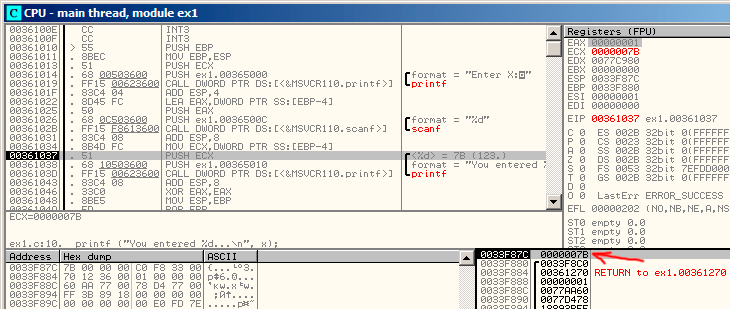
\includegraphics[scale=\FigScale]{patterns/04_scanf/ex1_olly_4.png}
\caption{\olly: \RU{готовим значение для передачи в}\EN{preparing the value for passing into} \printf}
\label{fig:scanf_ex1_olly_4}
\end{figure}

\subsection{GCC}

\RU{Попробуем тоже самое скомпилировать в Linux при помощи GCC 4.4.1:}
\EN{Let's try to compile this code in GCC 4.4.1 under Linux:}

\lstinputlisting{patterns/04_scanf/ex1_GCC.asm}

\index{puts() \RU{вместо}\EN{instead of} printf()}
\RU{GCC заменил первый вызов \printf на \puts, почему это было сделано, 
уже было описано раннее~(\ref{puts}).}
\EN{GCC replaced first the \printf call to the \puts, it was already described~(\ref{puts})
why it was done.}

% TODO: rewrite
%\RU{Почему \scanf переименовали в \TT{\_\_\_isoc99\_scanf}, я честно говоря, пока не знаю.}
%\EN{Why \scanf is renamed to \TT{\_\_\_isoc99\_scanf}, I do not know yet.}

\RU{Далее все как и прежде ~--- параметры заталкиваются через стек при помощи \MOV.}
\EN{As before~---arguments are placed on the stack by \MOV instruction.}

\subsection{x64}

\index{x86-64}
\IFRU{Всё то же самое, только используются регистры вместо стека для передачи аргументов функций}
{All the same, but registers are used instead of stack for arguments passing}.

\subsubsection{MSVC}

\lstinputlisting[caption=MSVC 2012 x64]{patterns/04_scanf/ex1_MSVC_x64.asm}

\subsubsection{GCC}

\lstinputlisting[caption=GCC 4.4.6 -O3 x64]{patterns/04_scanf/ex1_GCC_x64.s}


\section{ARM}

\subsection{\OptimizingKeil + \ThumbMode}

\begin{lstlisting}
.text:00000042             scanf_main
.text:00000042
.text:00000042             var_8           = -8
.text:00000042
.text:00000042 08 B5                       PUSH    {R3,LR}
.text:00000044 A9 A0                       ADR     R0, aEnterX     ; "Enter X:\n"
.text:00000046 06 F0 D3 F8                 BL      __2printf
.text:0000004A 69 46                       MOV     R1, SP
.text:0000004C AA A0                       ADR     R0, aD          ; "%d"
.text:0000004E 06 F0 CD F8                 BL      __0scanf
.text:00000052 00 99                       LDR     R1, [SP,#8+var_8]
.text:00000054 A9 A0                       ADR     R0, aYouEnteredD___ ; "You entered %d...\n"
.text:00000056 06 F0 CB F8                 BL      __2printf
.text:0000005A 00 20                       MOVS    R0, #0
.text:0000005C 08 BD                       POP     {R3,PC}
\end{lstlisting}

\index{\CLanguageElements!\Pointers}
\IFRU{Чтобы \scanf мог вернуть значение, ему нужно передать указатель на переменную типа \Tint.}
{A pointer
to a \Tint-typed variable must be passed to a \scanf so it can return value via it.}
\Tint \IFRU{~--- 32-битное значение, для его хранения нужно только 4 байта, и оно помещается в 
32-битный регистр.}
{is 32-bit value, so we need 4 bytes for storing it somewhere in memory, and it fits exactly 
in 32-bit register.}
\index{IDA!var\_?}
\IFRU{Место для локальной переменной \TT{x} выделяется в стеке, \IDA наименовала её \IT{var\_8}, 
впрочем, место для нее выделять не обязательно, т.к., \glslink{stack pointer}{указатель стека} \ac{SP} уже указывает на место, 
свободное для использования сразу же.}{A place for the local variable \TT{x} is allocated in the stack and \IDA
named it \IT{var\_8}, however, it is not necessary to allocate it since \ac{SP} \gls{stack pointer}
is already pointing to the space may be used instantly.}
\IFRU{Так что значение указателя \ac{SP} копируется в регистр \Reg{1}, и вместе с format-строкой, 
передается в \scanf.}
{So, \ac{SP} \gls{stack pointer} value is copied to the \Reg{1} register and, together with format-string, passed
into \scanf.}
\index{ARM!\Instructions!LDR}
\IFRU{Позже, при помощи инструкции \TT{LDR}, это значение перемещается из стека в регистр \Reg{1}, 
чтобы быть переданным в \printf.}{Later, with the help of the \TT{LDR} instruction, this value is moved
from stack into the \Reg{1} register in order to be passed into \printf.}

\IFRU{Варианты, скомпилированные для ARM-режима процессора, а также варианты скомпилированные при 
помощи Xcode LLVM, не очень отличаются от этого, так что, мы можем пропустить их здесь.}
{Examples compiled for ARM-mode and also examples compiled with Xcode LLVM are not differ significantly
from what we saw here, so they are omitted.}



\section{\RU{Глобальные переменные}\EN{Global variables}}
\index{\RU{Глобальные переменные}\EN{Global variables}}
\label{scanf_global_variable}

\RU{А что если переменная \TT{x} из предыдущего примера будет глобальной переменной, а не локальной? 
Тогда к ней смогут обращаться из любого другого места, а не только из тела функции. 
Глобальные переменные считаются \glslink{anti-pattern}{анти-паттерном},
но ради примера мы можем себе это позволить.}
\EN{What if \TT{x} variable from previous example will not be local but global variable? 
Then it will be accessible from any point, not only from function body. 
Global variables are considered as \gls{anti-pattern}, but for the sake of experiment we could do this.}

\lstinputlisting{patterns/04_scanf/ex2.c}

\subsection{MSVC: x86}

\lstinputlisting{patterns/04_scanf/ex2_MSVC.asm}

\RU{Ничего особенного, в целом. Теперь \TT{x} объявлена в сегменте \TT{\_DATA}. 
Память для нее в стеке более не выделяется.
Все обращения к ней происходит не через стек, а уже напрямую. 
Неинициализированные глобальные переменные не занимают места в исполняемом файле
(и действительно, зачем в исполняемом файле
нужно выделять место под изначально нулевые переменные?), но тогда, когда к этому месту в памяти
кто-то обратится, \ac{OS} подставит туда блок состоящий из нулей\footnote{Так работает \ac{VM}}.}
\EN{Now \TT{x} variable is defined in the \TT{\_DATA} segment. 
Memory in local stack is not allocated anymore. 
All accesses to it are not via stack but directly to process memory. 
Not initialized global variables takes no place in the executable file
(indeed, why we should allocate a place
in the executable file for initially zeroed variables?), but when someone will access this place
in memory, \ac{OS} will allocate a block of zeroes there\footnote{That is how \ac{VM} behaves}.}

\RU{Попробуем изменить объявление этой переменной:}
\EN{Now let's assign value to variable explicitly:}

\begin{lstlisting}
int x=10; // default value
\end{lstlisting}

\RU{Выйдет в итоге:}\EN{We got:}

\begin{lstlisting}
_DATA	SEGMENT
_x	DD	0aH

...
\end{lstlisting}

\RU{Здесь уже по месту этой переменной записано \TT{0xA} с типом DD (dword = 32 бита).}
\EN{Here we see value \TT{0xA} of DWORD type (DD meaning DWORD = 32 bit).}

\RU{Если вы откроете скомпилированный .exe-файл в \IDA, то увидите что \IT{x} 
находится аккурат в начале сегмента \TT{\_DATA}, после этой переменной будут текстовые строки.}
\EN{If you will open compiled .exe in \IDA, you will see the \IT{x} variable placed at the beginning of 
the \TT{\_DATA} segment, and after you'll see text strings.}

\RU{А вот если вы откроете в \IDA, .exe скомпилированный в прошлом примере, 
где значение \IT{x} не определено, то в IDA вы увидите:}
\EN{If you will open compiled .exe in \IDA from previous example where \IT{x} value is not defined, 
you'll see something like this:}

\begin{lstlisting}
.data:0040FA80 _x              dd ?                    ; DATA XREF: _main+10
.data:0040FA80                                         ; _main+22
.data:0040FA84 dword_40FA84    dd ?                    ; DATA XREF: _memset+1E
.data:0040FA84                                         ; unknown_libname_1+28
.data:0040FA88 dword_40FA88    dd ?                    ; DATA XREF: ___sbh_find_block+5
.data:0040FA88                                         ; ___sbh_free_block+2BC
.data:0040FA8C ; LPVOID lpMem
.data:0040FA8C lpMem           dd ?                    ; DATA XREF: ___sbh_find_block+B
.data:0040FA8C                                         ; ___sbh_free_block+2CA
.data:0040FA90 dword_40FA90    dd ?                    ; DATA XREF: _V6_HeapAlloc+13
.data:0040FA90                                         ; __calloc_impl+72
.data:0040FA94 dword_40FA94    dd ?                    ; DATA XREF: ___sbh_free_block+2FE
\end{lstlisting}

\RU{\TT{\_x} обозначен как \TT{?}, наряду с другими переменными не требующими инициализации. 
Это означает, что при загрузке .exe в память, место под все это выделено будет и будет заполнено
нулевыми байтами \cite[6.7.8p10]{C99TC3}. 
Но в самом .exe ничего этого нет. Неинициализированные переменные не занимают места в исполняемых файлах. 
Удобно для больших массивов, например.}
\EN{\TT{\_x} marked as \TT{?} among other variables not required to be initialized. 
This means that after loading .exe to memory, a space for all these variables will be 
allocated and filled by zeroes \cite[6.7.8p10]{C99TC3}. 
But in an .exe file these not initialized variables are not occupy anything. 
E.g. it is suitable for large arrays.}

\subsection{MSVC: x86 + \olly}
\index{\olly}

\RU{Тут даже проще}\EN{Things are even simpler here}: \figref{fig:scanf_ex2_olly_1}.
\RU{Переменная хранится в сегменте данных}\EN{Variable is located in the data segment}.
\RU{Кстати, после исполнения инструкции \PUSH (заталкивающей адрес $x$) адрес появится в стеке, и на этом
элементе можно нажать правой кнопкой, выбрать ``Follow in dump''}\EN{By the way, after 
\PUSH instruction (pushing $x$ address) is executed, the address
will appear in stack, and it is possible to right-click on that element and select ``Follow in dump''}.
\RU{И в окне памяти слева появится эта переменная}\EN{And the variable will appear in the memory window
at left}.

\RU{После того как в консоли введем 123, здесь появится}\EN{After we enter 123 in the console,} 
\TT{0x7B}\EN{ will appear here}.

\RU{Почему самый первый байт это}\EN{But why the very first byte is} \TT{7B}?
\RU{По логике вещей, здесь должно было бы быть}\EN{Thinking logically, a} \TT{00 00 00 7B}\EN{ should be
there}.
\RU{Это называется}\EN{This is what called} \gls{endianness}, \RU{и в x86 принят формат}\EN{and} 
\IT{little-endian}\EN{ is used in x86}.
\RU{Это означает что в начале записывается самый младший байт, а заканчивается самым старшим байтом}
\EN{This mean that lowest byte is written first, and highest written last}.
\RU{Больше об этом}\EN{More about it}: \ref{sec:endianness}.

\RU{Позже, из этого места в памяти, 32-битное значение загружается в \EAX и передается в}
\EN{Some time after, 32-bit value from this place of memory is loaded into \EAX and passed into} \printf.

\RU{Адрес переменной $x$ в памяти}\EN{$x$ variable address in the memory is} \TT{0xDC3390}.
\RU{В \olly{} мы можем посмотреть карту памяти процесса (Alt-M) и увидим что этот адрес
внутри PE-сегмента \TT{.data} нашей программы}\EN{In \olly we can see process memory map (Alt-M)
and we will see that this address is inside of \TT{.data} PE-segment of our program}:
\figref{fig:scanf_ex2_olly_2}.

\begin{figure}[H]
\centering
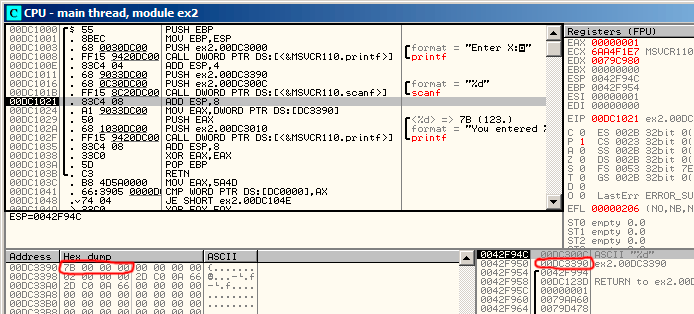
\includegraphics[scale=\FigScale]{patterns/04_scanf/ex2_olly_1.png}
\caption{\olly: \RU{после исполнения \scanf}\EN{after \scanf execution}}
\label{fig:scanf_ex2_olly_1}
\end{figure}

\begin{figure}[H]
\centering
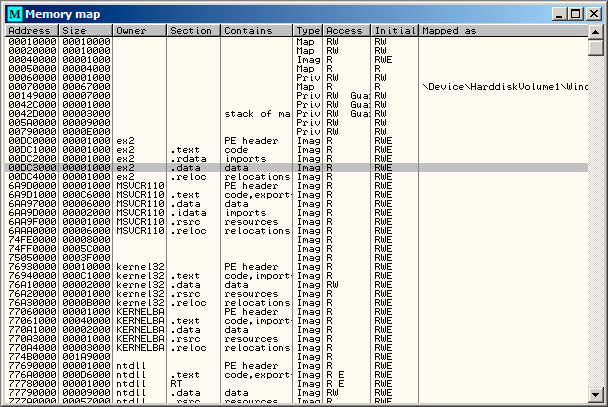
\includegraphics[scale=\FigScale]{patterns/04_scanf/ex2_olly_2.png}
\caption{\olly: \RU{карта памяти процесса}\EN{process memory map}}
\label{fig:scanf_ex2_olly_2}
\end{figure}

\subsection{GCC: x86}

\index{ELF}
\RU{В Linux все также почти. За исключением того, что если значение \TT{x} не определено, 
то эта переменная будет находится в сегменте \TT{\_bss}.
В \ac{ELF} этот сегмент имеет такие атрибуты:}
\EN{It is almost the same in Linux, except segment names and properties: 
not initialized variables are located in the \TT{\_bss} segment. 
In \ac{ELF} file format this segment has such attributes:}

\begin{lstlisting}
; Segment type: Uninitialized
; Segment permissions: Read/Write
\end{lstlisting}

\RU{Ну а если сделать статическое присвоение этой переменной какого-либо
значения, например, $10$, то она будет находится 
в сегменте \TT{\_data},
это сегмент с такими атрибутами:}
\EN{If to statically assign a value to variable, e.g. $10$, it will be placed in the \TT{\_data} segment, 
this is segment with the following attributes:}

\begin{lstlisting}
; Segment type: Pure data
; Segment permissions: Read/Write
\end{lstlisting}

\subsection{MSVC: x64}

\lstinputlisting[caption=MSVC 2012 x64]{patterns/04_scanf/ex2_MSVC_x64.asm}

\RU{Почти такой же код как и в}\EN{Almost the same code as in} x86.
\RU{Обратите внимание что для \TT{scanf()} адрес переменной $x$ передается
при помощи инструкции \LEA, а во второй \printf передается само значение переменной при помощи \MOV}
\EN{Take a notice that $x$ variable address is passed to \TT{scanf()} using \LEA instruction,
while the value of variable is passed to the second \printf using \MOV instruction}.
\TT{``DWORD PTR''}\EMDASH{}\RU{это часть языка ассемблера (не имеющая отношения к машинным кодам) 
показывающая, что тип переменной в памяти\EMDASH{}именно 32-битный, 
и инструкция \MOV должна быть здесь закодирована соответственно}\EN{is a part of assembly language 
(no related to machine codes), showing that the variable data type is 32-bit and the \MOV instruction
should be encoded accordingly}.



\subsection{ARM: \OptimizingKeilVI + \ThumbMode}

\begin{lstlisting}
.text:00000000 ; Segment type: Pure code
.text:00000000                 AREA .text, CODE
...
.text:00000000 main
.text:00000000                 PUSH    {R4,LR}
.text:00000002                 ADR     R0, aEnterX     ; "Enter X:\n"
.text:00000004                 BL      __2printf
.text:00000008                 LDR     R1, =x
.text:0000000A                 ADR     R0, aD          ; "%d"
.text:0000000C                 BL      __0scanf
.text:00000010                 LDR     R0, =x
.text:00000012                 LDR     R1, [R0]
.text:00000014                 ADR     R0, aYouEnteredD___ ; "You entered %d...\n"
.text:00000016                 BL      __2printf
.text:0000001A                 MOVS    R0, #0
.text:0000001C                 POP     {R4,PC}
...
.text:00000020 aEnterX         DCB "Enter X:",0xA,0    ; DATA XREF: main+2
.text:0000002A                 DCB    0
.text:0000002B                 DCB    0
.text:0000002C off_2C          DCD x                   ; DATA XREF: main+8
.text:0000002C                                         ; main+10
.text:00000030 aD              DCB "%d",0              ; DATA XREF: main+A
.text:00000033                 DCB    0
.text:00000034 aYouEnteredD___ DCB "You entered %d...",0xA,0 ; DATA XREF: main+14
.text:00000047                 DCB 0
.text:00000047 ; .text         ends
.text:00000047
...
.data:00000048 ; Segment type: Pure data
.data:00000048                 AREA .data, DATA
.data:00000048                 ; ORG 0x48
.data:00000048                 EXPORT x
.data:00000048 x               DCD 0xA                 ; DATA XREF: main+8
.data:00000048                                         ; main+10
.data:00000048 ; .data         ends
\end{lstlisting}

\RU{Итак, переменная \TT{x} теперь глобальная, и она расположена, почему-то, в другом сегменте, 
а именно сегменте данных}\EN{So, \TT{x} variable is now global and somehow,
it is now located in another segment, namely data segment} (\IT{.data}).
\RU{Можно спросить, почему текстовые строки расположены в сегменте кода (\IT{.text}) 
а \TT{x} нельзя было разместить тут же?}\EN{One could ask, why text strings are located in code segment
(\IT{.text}) and \TT{x} can be located right here?}
\RU{Потому что эта переменная, и как следует из определения, она может меняться. 
И может даже быть, меняться часто.}
\EN{Since this is variable, and by its definition, it can be changed. And probably, can be changed 
very often.}
\index{\RAM}
\index{\ROM}
\RU{Сегмент кода нередко может быть расположен в ПЗУ микроконтроллера (не забывайте, 
мы сейчас имеем дело с embedded-микроэлектроникой, где дефицит памяти ~--- это обычное дело),
а изменяемые переменные ~--- в ОЗУ.}
\EN{Segment of code not infrequently can be located in microcontroller ROM (remember, we now deal
with embedded microelectronics, and memory scarcity is common here), and changeable 
variables~---in \ac{RAM}.}
\RU{Хранить в ОЗУ неизменяемые данные, когда в наличии есть ПЗУ, не экономно.}
\EN{It is not very economically to store constant variables in RAM when one have ROM.}
\RU{К тому же, сегмент данных в ОЗУ с константами нужно было бы инициализировать перед работой,
ведь, после включения ОЗУ, очевидно, она содержит в себе случайную информацию.}
\EN{Furthermore, data segment with constants in RAM must be initialized before, 
since after RAM turning on, obviously, it contain random information.}

\index{\RU{Компоновщик}\EN{Linker}}
\RU{Далее, мы видим, в сегменте кода, хранится указатель на переменную \TT{x} (\TT{off\_2C}) и вообще, 
все операции с переменной, происходят через этот указатель.}
\EN{Onwards, we see, in code segment, a pointer to the \TT{x} (\TT{off\_2C}) variable, and all
operations with variable occurred via this pointer.}
\RU{Это связано с тем что переменная \TT{x} может быть расположена где-то довольно далеко от 
данного участка кода, так что её адрес нужно сохранить в непосредственной близости к этому коду.}
\EN{This is because \TT{x} variable can be located somewhere far from this code fragment, so its address
must be saved somewhere in close proximity to the code.}
\index{ARM!\Instructions!LDR}
\RU{Инструкция \TT{LDR} в thumb-режиме может адресовать только переменные в пределах вплоть 
до 1020 байт от места где она находится.}
\EN{\TT{LDR} instruction in thumb mode can address only variable in range of 1020 bytes from the point
it is located.}
\RU{Эта же инструкция в ARM-режиме ~--- переменные в пределах $\pm{}4095$ байт, таким образом,
адрес глобальной переменной \TT{x} нужно расположить в непосредственной близости, ведь нет никакой гарантии, 
что компоновщик\footnote{linker в англоязычной литературе} сможет разместить саму переменную где-то рядом, 
она может быть даже в другом чипе памяти!}
\EN{Same instruction in ARM-mode~---variables in range $\pm{}4095$ bytes, this, address of the \TT{x} variable
must be located somewhere in close proximity, because, there is no guarantee the linker will able to place
this variable near the code, it could be even in external memory chip!}

\index{\CLanguageElements!const}
\index{\ROM}
\RU{Еще одна вещь: если переменную объявить как \IT{const}, то компилятор Keil разместит её в 
сегменте \TT{.constdata}.}
\EN{One more thing: if variable will be declared as \IT{const}, Keil compiler shall allocate it in 
the \TT{.constdata} segment.}
\RU{Должно быть, впоследствии, компоновщик и этот сегмент сможет разместить в ПЗУ, вместе
с сегментом кода.}
\EN{Perhaps, thereafter, linker will able to place this segment in ROM too, along with code segment.}



\section{\RU{Проверка результата scanf()}\EN{scanf() result checking}}

\RU {Как я уже упоминал, использовать \scanf в наше время это слегка старомодно. 
Но если уж жизнь заставила этим заниматься, нужно хотя бы проверять, сработал ли \scanf 
правильно или пользователь ввел вместо числа что-то другое, что \scanf не смог трактовать как число.}
\EN{As I noticed before, it is slightly old-fashioned to use \scanf today. 
But if we have to, we need at least check if \scanf finished correctly without error.}

\lstinputlisting{patterns/04_scanf/ex3.c}

\RU{По стандарту}\EN{By standard}, 
\scanf\footnote{MSDN: scanf, wscanf: \url{http://msdn.microsoft.com/en-us/library/9y6s16x1(VS.71).aspx}} 
\RU{возвращает количество успешно полученных значений.}
\EN{function returns number of fields it successfully read.}

\RU{В нашем случае, если все успешно и пользователь ввел таки некое число, \scanf вернет 1. 
А если нет, то 0 (или EOF).} 
\EN{In our case, if everything went fine and user entered a number, 
\scanf will return 1 or 0 (or EOF) in case of error.}

\RU{Я добавил код проверяющий результат \scanf и в случае ошибки, он сообщает пользователю что-то другое.}
\EN{I added C code for \scanf result checking and printing error message in case of error.}

\RU{Это работает предсказуемо}\EN{This works predictably}:

\begin{lstlisting}
C:\...>ex3.exe
Enter X:
123
You entered 123...

C:\...>ex3.exe
Enter X:
ouch
What you entered? Huh?
\end{lstlisting}

\subsubsection{MSVC: x86}

\IFRU{Вот, что выходит на ассемблере}{What we got in assembly language} (MSVC 2010):

\lstinputlisting{patterns/04_scanf/ex3_MSVC_x86.asm}

\index{x86!\Registers!EAX}
\IFRU{Для того чтобы вызывающая функция имела доступ к результату вызываемой функции, 
вызываемая функция (в нашем случае \scanf) оставляет это значение в регистре \EAX.}
{\Gls{caller} function (\main) must have access to the result of \gls{callee} function (\scanf), 
so \gls{callee} leaves this value in the \EAX register.}

\index{x86!\Instructions!CMP}
\IFRU{Мы проверяем его инструкцией \TT{CMP EAX, 1} (\IT{CoMPare}), то есть, 
сравниваем значение в \EAX с 1.}
{After, we check it with the help of instruction \TT{CMP EAX, 1} (\IT{CoMPare}),
in other words, we compare value in the \EAX register with $1$.} 

\index{x86!\Instructions!JNE}
\IFRU{Следующий за инструкцией \CMP: условный переход \JNE. 
Это означает \IT{Jump if Not Equal}, то есть, условный переход \IT{если не равно}.}
{\JNE conditional jump follows \CMP instruction. \JNE means \IT{Jump if Not Equal}.}

\IFRU{Итак, если \EAX не равен 1, то \JNE заставит перейти процессор 
по адресу указанном в операнде \JNE, у нас это \TT{\$LN2@main}.}
{So, if value in the \EAX register not equals to $1$, then the processor will pass execution to the 
address mentioned in operand of \JNE, in our case it is \TT{\$LN2@main}.}
\IFRU
{Передав управление по этому адресу, \ac{CPU} как раз начнет исполнять вызов \printf с 
аргументом \TT{``What you entered? Huh?''}.}
{Passing control to this address, \ac{CPU} will execute function \printf 
with argument \TT{``What you entered? Huh?''}.}
\IFRU
{Но если все нормально, перехода не случится, и исполнится другой \printf с двумя аргументами: 
\TT{'You entered \%d...'} и значением переменной \TT{x}.}
{But if everything is fine, conditional jump will not be taken, and another \printf call 
will be executed, with two arguments: \TT{'You entered \%d...'} and value of variable \TT{x}. }

\index{x86!\Instructions!XOR}
\index{\CLanguageElements!return}
\IFRU {А для того чтобы после этого вызова не исполнился сразу второй вызов \printf, 
после него имеется инструкция \JMP, безусловный переход, он отправит процессор на место аккурат 
после второго \printf и перед инструкцией \TT{XOR EAX, EAX}, которая собственно \TT{return 0}.}
{Since second subsequent \printf not needed to be executed, there is \JMP after (unconditional jump),
it will pass control to the point after second \printf and before \TT{XOR EAX, EAX} instruction, 
which implement \TT{return 0}.}

\index{x86!\Registers!\Flags}
\IFRU{Итак, можно сказать, что в подавляющих случаях сравнение какой-либо переменной с чем-то другим 
происходит при помощи пары инструкций \CMP и \Jcc, где \IT{cc} это \IT{condition code}.}
{So, it can be said that comparing a value with another is \IT{usually} implemented
by \CMP/\Jcc instructions pair, where \IT{cc} is \IT{condition code}.}
\IFRU{\CMP сравнивает два значения и выставляет 
флаги процессора\footnote{См. также о флагах x86-процессора: \url{http://en.wikipedia.org/wiki/FLAGS_register_(computing)}.}.}
{\CMP comparing two values and set 
processor flags\footnote{About x86 flags, see also: \url{http://en.wikipedia.org/wiki/FLAGS_register_(computing)}.}.}
\IFRU
{\Jcc проверяет нужные ему флаги и выполняет переход по указанному адресу (или не выполняет).}
{\Jcc check flags needed to be checked and pass control to mentioned address (or not pass).}

\index{x86!\Instructions!CMP}
\index{x86!\Instructions!SUB}
\label{CMPandSUB}
\IFRU{Но на самом деле, как это не парадоксально поначалу звучит, \CMP это почти то же самое что и 
инструкция \SUB, которая отнимает числа одно от другого.}
{But in fact, this could be perceived paradoxical, but \CMP instruction is in fact \SUB (subtract).}
\IFRU{Все арифметические инструкции также выставляют флаги в соответствии с результатом, не только \CMP.}
{All arithmetic instructions set processor flags too, not only \CMP.}
\IFRU{Если мы сравним 1 и 1, от единицы отнимется единица, получится $0$, и выставится флаг 
\ZF (\IT{zero flag}), означающий что последний полученный результат был $0$.}
{If we compare 1 and 1, $1-1$ will be $0$ in result, \ZF flag will be set (meaning the last result was $0$).}
\IFRU{Ни при каких других значениях \EAX, флаг \ZF выставлен не будет, кроме тех, когда операнды равны друг другу.}
{There is no any other circumstances when it is possible except when operands are equal.}
\index{x86!\Instructions!JNE}
\index{x86!\Registers!ZF}
\IFRU{Инструкция \JNE проверяет только флаг \ZF, и совершает переход только если флаг не поднят. 
Фактически, \JNE это синоним инструкции \JNZ (\IT{Jump if Not Zero}).}
{\JNE checks only \ZF flag and jumping only if it is not set. 
\JNE is in fact a synonym of \JNZ (\IT{Jump if Not Zero}) instruction.}
\IFRU{Ассемблер транслирует обе инструкции в один и тот же опкод.}
{Assembler translating both \JNE and \JNZ instructions into one single opcode.}
\IFRU
{Таким образом, можно \CMP заменить на \SUB и все будет работать также, но разница в том, что \SUB 
все-таки испортит значение в первом операнде. \CMP это \IT{SUB без сохранения результата}.}
{So, \CMP instruction can be replaced to \SUB instruction and almost everything will be fine,
but the difference is in 
the \SUB alter the value of the first operand.
\CMP is \IT{``SUB without saving result''}.}

\subsubsection{MSVC: x86: IDA}

\index{IDA}
\IFRU{Наверное, уже пора делать первые попытки анализа кода в \IDA}
{It's time to run \IDA and try to do something in it}.
\IFRU{Кстати, для начинающих, полезно компилировать в MSVC с ключом \TT{/MD}, что означает что все эти стандартные
ф-ции не будут скомпонованы с исполняемым файлу, а будут импортироваться из файла \TT{MSVCR*.DLL}}
{By the way, it is good idea to use \TT{/MD} option in MSVC for beginners: this mean that all these
standard functions will not be linked with executable file, but will be imported from the \TT{MSVCR*.DLL}
file instead}.
\IFRU{Так будет легче увидеть, где какая стандартная ф-ция используется}{Thus it will be easier to see
which standard function used and where}.

\IFRU{Анализируя код в \IDA, очень полезно делать пометки для себя (и других)}
{While analysing code in \IDA, it is very advisable to do notes for oneself (and others)}.
\IFRU{Например, разбирая этот пример, мы сразу видим что \TT{JNZ} срабатывает в случае ошибки}
{For example, analysing this example, we see that \TT{JNZ} will be triggered in case of error}.
\IFRU{Можно навести курсор на эту метку, нажать ``n'' и переименовать метку в ``error''}
{So it's possible to move cursor to the label, press ``n'' and rename it to ``error''}.
\IFRU{Еще одну метку}{Another label}\EMDASH{}\IFRU{в}{into} ``exit''.
\IFRU{Вот как у меня получилось в итоге}{What I've got}:

\lstinputlisting{patterns/04_scanf/ex3.lst}

\IFRU{Так понимать код становится чуть легче}{Now it's slightly easier to understand the code}.
\IFRU{Впрочем, меру нужно знать во всем и комментировать каждую инструкцию не стоит}
{However, it's not good idea to comment every instruction excessively}.

\IFRU{В \IDA также можно скрывать части ф-ций: нужно отметить часть, нажать ``-'' на цифровой клавиатуре и ввести
текст}{A part of function can also be hidden in \IDA: a block should be marked, then ``-'' on numerical pad
is pressed and text to be entered}.

\IFRU{Я скрыл две части и придумал им названия}{I've hide two parts and gave names to them}:

\lstinputlisting{patterns/04_scanf/ex3_2.lst}

\IFRU{Раскрывать скрытые части ф-ций можно при помощи ``+'' на цифровой клавиатуре}
{To unhide these parts, ``+'' on numerical pad can be used}.

\IFRU{Нажав ``пробел'', мы увидим как \IDA может представить ф-цию в виде графа}{By pressing ``space'',
we can see how \IDA can represent a function as a graph}: \figname{} \ref{fig:ex3_IDA_1}.
\IFRU{После каждого условного перехода видны две стрелки: зеленая и красная}{There are two arrows
after each conditional jump: green and red}.
\IFRU{Зеленая ведет к тому блоку, который исполнится если переход сработал, а красная --- если не сработал}
{Green arrow pointing to the block which will be executed if jump is triggered, and red if otherwise}.

\IFRU{В этом режиме так же можно сворачивать узлы и давать им названия}
{It is possible to fold nodes is this mode and give them names as well} (``group nodes'').
\IFRU{Я сделал это для трех блоков}{I did it for 3 blocks}: \figname{} \ref{fig:ex3_IDA_2}.

\IFRU{Всё это очень полезно делать}{It's very useful}.
\IFRU{Вообще, очень важная часть работы реверсера состоит в том, чтобы уменьшать количество имеющейся информации}
{It can be said, a very important part of reverse engineer's job is to reduce information he/she have}.

\begin{figure}[H]
\centering
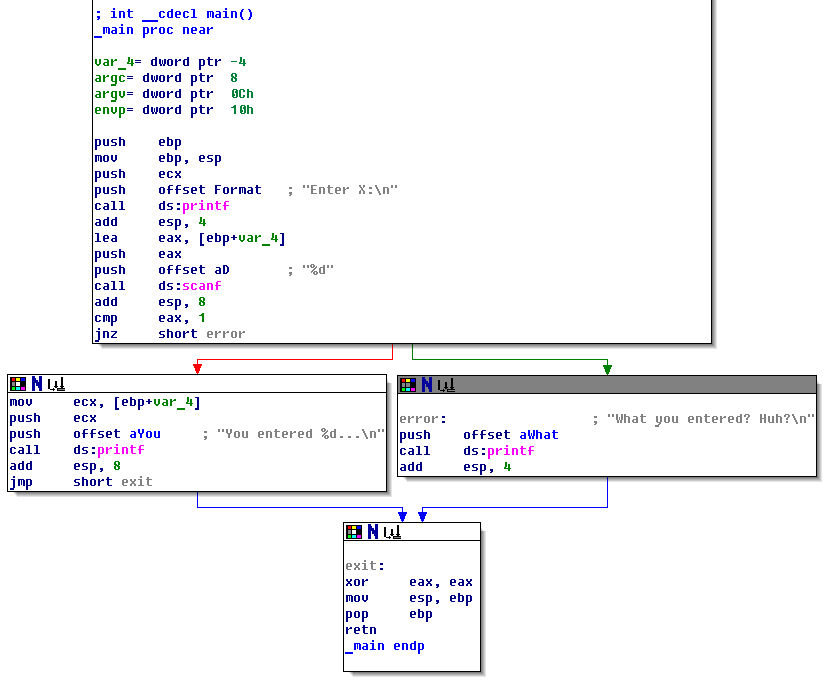
\includegraphics[scale=0.66]{patterns/04_scanf/ex3_IDA.png}
\caption{\IFRU{Отображение в IDA в виде графа}{Graph mode in IDA}}
\label{fig:ex3_IDA_1}
\end{figure}

\begin{figure}[H]
\centering
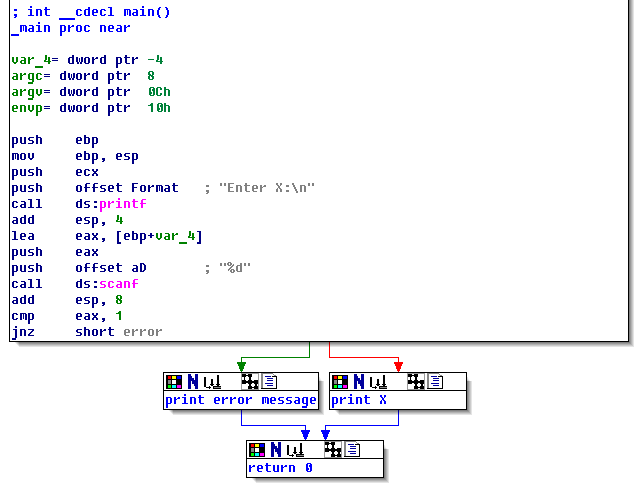
\includegraphics[scale=0.66]{patterns/04_scanf/ex3_2_IDA.png}
\caption{\IFRU{Отображение в IDA в виде графа с тремя свернутыми блоками}{Graph mode in IDA with 3 nodes folded}}
\label{fig:ex3_IDA_2}
\end{figure}

\subsubsection{MSVC: x86 + \olly}

\IFRU{Попробуем в \olly немного хакнуть программу, и сделать вид что \scanf срабатывает всегда без ошибок}
{Let's try to hack our program in \olly, forcing it to think \scanf working always without error}.

\IFRU{Когда в \scanf передается адрес локальной перемейнной, изначальное, в данном случае, 
у нас в этой переменной
находится некий мусор, а это}{When address of local variable is passed into \scanf,
initially this variable contain some random garbage, that is} \TT{0x4CD478}\EN{ in case}:
\figname \ref{fig:scanf_ex3_olly_1}.

\IFRU{Когда}{When} \scanf \IFRU{запускается, я ввожу в консоли что-то непохожее на число, например}
{is executing, I enter in the console something definitely not a number, like} ``asdasd''.
\scanf \IFRU{заканчивается с 0 в}{finishing with 0 in} \EAX, \IFRU{что означает, что произошла ошибка}
{which mean, an error occurred}: \figname \ref{fig:scanf_ex3_olly_2}.

\IFRU{Вместе с этим, мы можем посмотреть на локальную переменную в стеке, она не изменилась}
{We can also see to the local variable in the stack and notice that it's not changed}.
\IFRU{Действительно, ведь что туда записала бы ф-ция \scanf}{Indeed, what \scanf would write there}?
\IFRU{Она просто ничего не делала кроме возвращения нуля}{It just did nothing except returning zero}.

\IFRU{Теперь попробуем немного ``хакнуть'' нашу программу}{Now let's try to ``hack'' our program}.
\IFRU{Кликнем правой кнопкой на}{Let's right-click on} \EAX, \IFRU{там, в числе опций, будет также}
{there will also be} ``Set to 1''\EN{ among other options}.
\IFRU{Это то что нам нужно}{This is what we need}.

\IFRU{В \EAX теперь 1, последующая проверка пройдет как надо, и \printf выведет значение переменной
из стека}{1 now in \EAX, so the following check will executed as we need, and \printf will print
value of variable in the stack}.

\IFRU{Запускаем}{Let's run} (F9) \IFRU{и видим в консоли следующее}{and we will see this in 
console window}:

\begin{figure}[H]
\centering
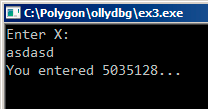
\includegraphics[scale=0.66]{patterns/04_scanf/ex3_olly_3.png}
\caption{\IFRU{консоль}{console window}}
\end{figure}

\IFRU{Действительно}{Indeed}, $5035128$ \IFRU{это десятичное представление числа в стеке}
{is a decimal representation of the number in stack} (\TT{0x4CD478})!

\begin{figure}[H]
\centering
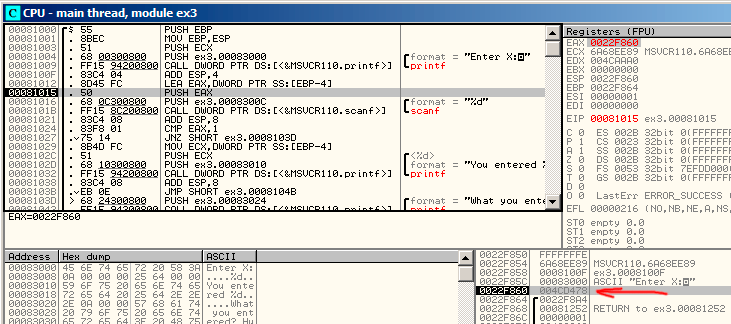
\includegraphics[scale=0.66]{patterns/04_scanf/ex3_olly_1.png}
\caption{\olly: \IFRU{передача адреса переменной в}{passing variable address into} \scanf}
\label{fig:scanf_ex3_olly_1}
\end{figure}

\begin{figure}[H]
\centering
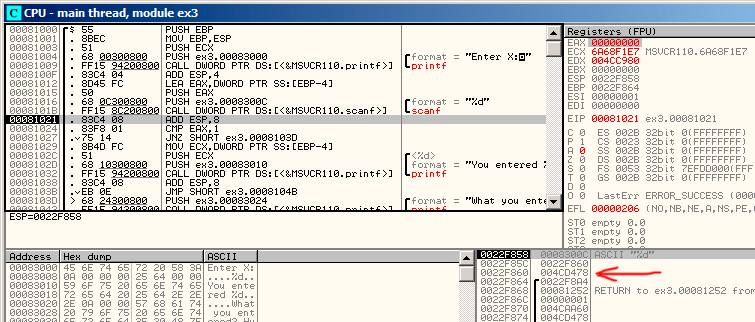
\includegraphics[scale=0.66]{patterns/04_scanf/ex3_olly_2.png}
\caption{\olly: \scanf \IFRU{закончился с ошибкой}{returning error}}
\label{fig:scanf_ex3_olly_2}
\end{figure}

\subsubsection{MSVC: x86 + Hiew}
\index{Hiew}

\IFRU{Это еще и может быть простым примером патчинга исполняемого файла}{This can be 
also a simple example of executable file patching}.
\IFRU{Мы можем попробовать пропатчить его таким образом, что программа всегда будет выводить числа,
вне зависимости от того, что мы вводим}{We may try to patch executable, so the program will always 
print numbers, no matter what we entered}.

\IFRU{Учитывая, что исполняемый файл скомпилирован с учетом импортирования ф-ций из}{Assuming the 
executable compiled against external} \TT{MSVCR*.DLL} (\IFRU{т.е., с опцией}{i.e., with} 
\TT{/MD}\EN{ option})\footnote{\IFRU{то, что еще называют}{that's what also called} ``dynamic linking''}, 
\IFRU{мы можем отыскать ф-цию}{we may find} \main \IFRU{в самом начале секции}{function at the 
very beginning of} \TT{.text}\EN{ section}.
\IFRU{Откроем исполняемый файл в Hiew, найдем самое начало секции}{Let's open executable in Hiew, 
find the very beginning of} \TT{.text}\EN{ section} (Enter, F8, F6, Enter, Enter).

\IFRU{Мы увидим следующее}{We will see this}: \figname \ref{fig:scanf_ex3_hiew_1}.

Hiew \IFRU{находт}{finds} \ac{ASCIIZ}\IFRU{-строки и показывает их, так же как и имена импортируемых 
ф-ций}{ strings and displays them, as well as imported function names}.

\IFRU{Переведите курсор на адрес}{Move cursor to the address} \TT{.00401027} 
(\IFRU{с инструкцией}{with the} \TT{JNZ}\IFRU{, которую мы хотим заблокировать}{ instruction we 
should bypass}), \IFRU{нажмите}{press} F3,
\IFRU{затем наберите}{and then type} ``9090'' (\IFRU{что означает}{meaning two} \ac{NOP}-\IFRU{а}{s}): 
\figname \ref{fig:scanf_ex3_hiew_2}.

\IFRU{Затем}{Then} F9 (update). \IFRU{Теперь исполняемый файл записан на диск. Он будет вести себя
так, как нам надо.}{Now the executable saved to disk. It will behave as we wanted.}

\IFRU{Два}{Two} \ac{NOP}-\IFRU{а}{s} \IFRU{возможно, не так эстетично, как могло бы быть}{are probably 
not quite \ae{}sthetically as it could be}.
\IFRU{Другой способ пропатчить инструкцию, это записать 0 во второй байт опкода (смещение перехода),
так что}{Other way to patch this instruction is to write just 0 to the second opcode byte (jump offset), 
so that} \TT{JNZ} \IFRU{всегда будет переходить на следующую инструкцию}{will always jump to 
the next instruction}.

\begin{figure}[H]
\centering
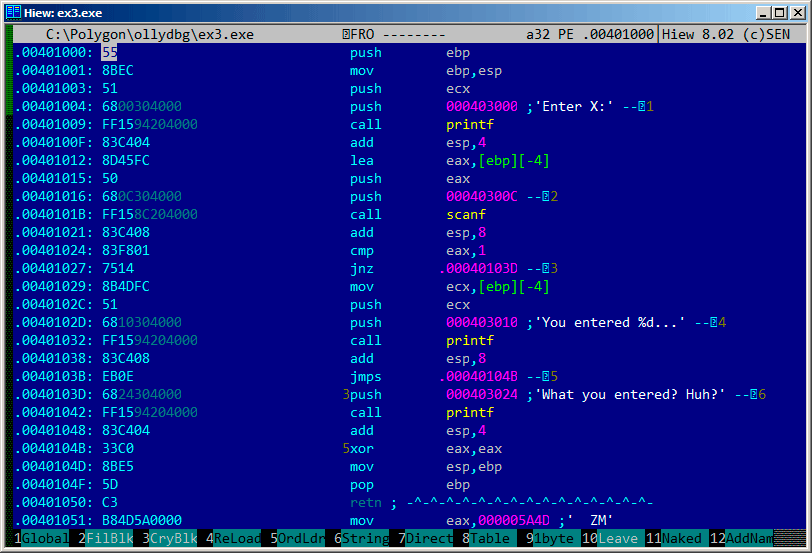
\includegraphics[scale=0.66]{patterns/04_scanf/ex3_hiew_1.png}
\caption{Hiew: \RU{ф-ция }\main\EN{ function}}
\label{fig:scanf_ex3_hiew_1}
\end{figure}

\begin{figure}[H]
\centering
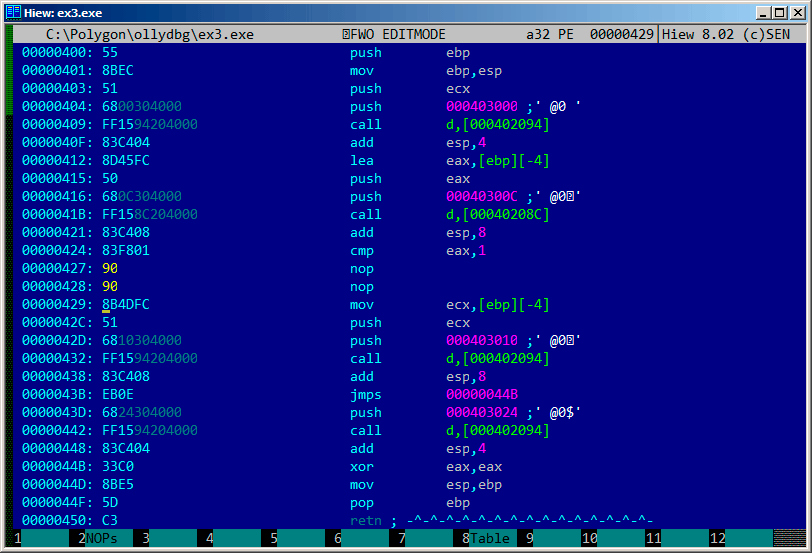
\includegraphics[scale=0.66]{patterns/04_scanf/ex3_hiew_2.png}
\caption{Hiew: \IFRU{замена}{replacing} \TT{JNZ} \IFRU{на два}{by two} \ac{NOP}-\IFRU{а}{s}}
\label{fig:scanf_ex3_hiew_2}
\end{figure}

\subsubsection{GCC: x86}

\IFRU{Код созданный при помощи GCC 4.4.1 в Linux практически такой же, если не считать мелких отличий, 
которые мы уже рассмотрели раннее.}
{Code generated by GCC 4.4.1 in Linux is almost the same, except differences we already considered.}

\subsection{MSVC: x64}

\index{x86-64}
\IFRU{Так как мы работаем здесь с переменными типа \Tint, а они в x86-64 остались 32-битными, то мы здесь видим
как продолжают использоваться регистры с префиксом \TT{E-}}{Since we work here with \Tint{}-typed variables,
which are still 32-bit in x86-64, we see how 32-bit part of registers (prefixed with \TT{E-}) 
are used here as well}.
\IFRU{Но для работы с указателями, конечно, используются 64-битные части регистров, с префиксом \TT{R-}}
{While working with pointers, however, 64-bit register parts are used, prefied with \TT{R-}}.

\lstinputlisting[caption=MSVC 2012 x64]{patterns/04_scanf/ex3_MSVC_x64.asm}


\ifdefined\IncludeARM
\subsubsection{ARM: \OptimizingKeil + \ThumbMode}

\lstinputlisting[caption=\OptimizingKeil + \ThumbMode]{patterns/04_scanf/ex3_ARM_Keil_thumb_O3.asm}

\index{ARM!\Instructions!CMP}
\index{ARM!\Instructions!BEQ}
\IFRU{Новые инструкции здесь для нас: \CMP и \ac{BEQ}.}
{New instructions here are \CMP and \ac{BEQ}.}

\CMP \IFRU{аналогична той что в x86, она отнимает один аргумент от второго и сохраняет флаги.}
{is akin to the x86 instruction bearing the same name, it subtracts one argument from another and saves flags.}
% TODO: в мануале ARM $op1 + NOT(op2) + 1$ вместо вычитания

\index{ARM!\Registers!Z}
\index{x86!\Instructions!JZ}
\ac{BEQ} \IFRU{совершает переход по другому адресу, 
если операнды при сравнении были равны, 
либо если результат последнего вычисления был $0$, либо если флаг Z равен $1$.}
{is jumping to another address if operands while comparing were equal to each other, or,
if result of last computation was $0$, or if Z flag is $1$.}
\IFRU{То же что и \JZ в}{Same thing as \JZ in} x86.

\IFRU{Всё остальное просто: исполнение разветвляется на две ветки, затем они сходятся там, 
где в \Reg{0} записывается $0$ как возвращаемое из функции значение и происходит выход из функции.}
{Everything else is simple: execution flow is forking into two branches, then the branches are 
converging at the point
where $0$ is written into the \Reg{0}, as a value returned from the function, and then function finishing.}


\fi


